\documentclass[a4paper,11pt]{article}
\input{/home/tof/Documents/Cozy/latex-include/preambule_lua.tex}
\newcommand{\showprof}{show them}  % comment this line if you don't want to see todo environment
\fancyhead[L]{Type construit - documentation}
\newdate{madate}{10}{09}{2020}
\fancyhead[R]{Première - NSI} %\today
\fancyfoot[L]{~\\Christophe Viroulaud}
\fancyfoot[C]{\textbf{Page \thepage}}
\fancyfoot[R]{\includegraphics[width=2cm,align=t]{/home/tof/Documents/Cozy/latex-include/cc.png}}

\begin{document}
\begin{Form}
\section{Langage de haut niveau}
Nous l'avons déjà évoqué, Python est un langage de haut niveau c'est à dire qu'il met à disposition des outils optimisés facilitant la vie du développeur. Par exemple la méthode \emph{len} renvoie la taille de la séquence donnée en paramètre (code \ref{len}).
\begin{code}[!h]
\begin{lstlisting}
>>> t = (1, 4, 8)
>>> len(t)
>>> 3
>>> l = [2, 6, 9, 10]
>>> len(l)
>>> 4
>>> texte = "bonjour"
>>> len(texte)
>>> 7
\end{lstlisting}
\captionof{code}{La méthode \emph{len} est utilisable avec plusieurs types de données}
\label{len}
\end{code}

Comparativement au langage machine que nous avons utilisé en début d'année nous n'avons par exemple pas besoin de gérer les appels mémoires.\\
Il est illusoire et de toute façon inutile de connaître toutes les fonctionnalités par cœur. Par contre il faut savoir les retrouver. La documentation est donc un outil précieux. Concentrons-nous sur la documentation des tableaux (les \emph{list} en Python).
\begin{center}
\url{https://docs.python.org/fr/3/tutorial/datastructures.html}
\end{center}
\section{Méthodes courantes}
Pour fixer les idées il est utile de visualiser ce qui se passe en mémoire. Le site \url{http://pythontutor.com/} simule l'exécution d'un programme Python. Nous utiliserons ce site pour la suite des activités.\\
Il faut cliquer sur \emph{Start visualizing your code now}.
\subsection{Comprendre la documentation}
La documentation donne le nom de la méthode et les \emph{paramètres} éventuels.

\shadowbox{\parbox{16cm}{
\textbf{list.pop([i])}\\
Enlève de la liste l'élément situé à la position indiquée et le renvoie en valeur de retour. Si aucune position n'est spécifiée, a.pop() enlève et renvoie le dernier élément de la liste.
}}

Dans cet exemple, il faut remarquer que:
\begin{itemize}
\item La méthode \emph{renvoie} la valeur dans le programme principal. Il est donc possible de la stocker dans une variable.
\item Le paramètre \emph{i} est facultatif. La notation par crochets indique ce caractère.
\end{itemize}
\begin{activite}
\begin{enumerate}
\item Créer une liste \textbf{l} de cinq entiers.
\item Enlever le dernier élément et le récupérer dans une variable \textbf{dernier}.
\item Enlever le premier élément et le récupérer dans une variable \textbf{premier}.
\end{enumerate}
\end{activite}

\subsection{Modifier un tableau}
Certaines opérations sont très courantes sur un tableau. Python offre des méthodes pour les réaliser.
\begin{activite}
\begin{enumerate}
\item Créer un tableau vide nommés \textbf{disciplines}.
\item Ajouter (une à une) les noms des disciplines étudiées en première.
\item Trier le tableau par ordre alphabétique.
\item Trouver l'indice de la discipline "NSI".
\item Supprimer une des trois spécialités.
\end{enumerate}
\end{activite}
\paragraph{Observation:} Il faut remarquer que derrière ces méthodes simples d'utilisation se cachent des algorithmes parfois complexes. Nous y reviendrons plus tard dans l'année.
\subsection{Copier un tableau}
\begin{activite}
\begin{enumerate}
\item Tester le code suivant. Le comportement a déjà été observé dans les cours précédents.
\begin{lstlisting}
a = 3
b = 4
a = b
a = 5
\end{lstlisting}
\item Tester le code suivant.
\begin{lstlisting}
l1 = [1, 2, 3]
l2 = l1
l1[0] = 4
\end{lstlisting}
En première approche nous pouvons expliquer ce comportement ainsi: la variable \emph{l1} ne contient pas le tableau mais \emph{l'adresse mémoire} de ce dernier. La variable \emph{l2} \emph{pointe} alors vers le même espace mémoire que \emph{l1}.
\item Dans la documentation, trouver une méthode qui permet de créer une vraie copie de \emph{l1}.
\end{enumerate}
\end{activite}
\subsection{Itérer sur un tableau}
C'est une opération courante sur un tableau. Il existe plusieurs manières de réaliser cette itération. 
\begin{activite}
\begin{enumerate}
\item Écrire une boucle qui affiche les disciplines entrées dans le tableau \emph{disciplines}.
\item Tester le code suivant. Bien prendre le temps de comprendre cette implémentation.
\begin{lstlisting}
for matiere in disciplines:
	print(matiere, end=" ")
\end{lstlisting}
\end{enumerate}
\end{activite}
\section{Des tableaux plus complexes}
Nous avons crée des tuples et des tableaux d'entiers (\emph{int}) ou de chaînes de caractère (\emph{string}) mais il est possible de stocker des objets plus complexes. Imaginons un programme qui implémente le jeu \emph{Puissance 4}. Le plateau de jeu (figure \ref{puissance4}) est composé de six lignes de sept colonnes.
\begin{figure}[!h]
\centering
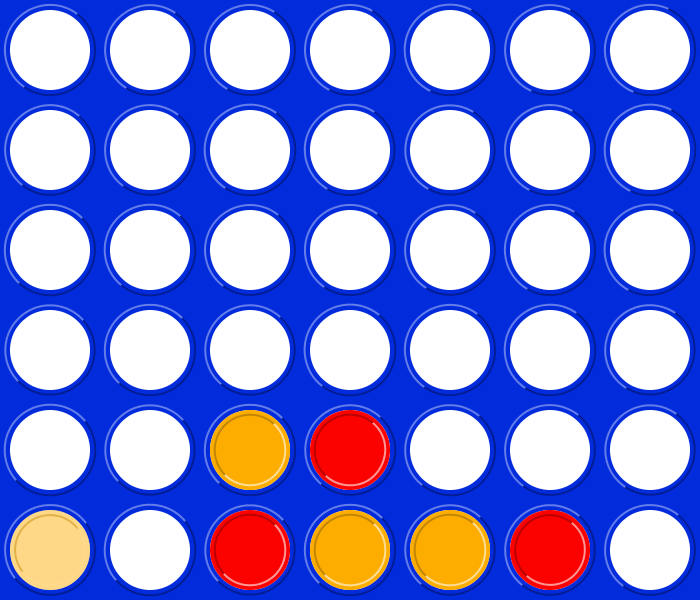
\includegraphics[width=7cm]{ressources/puissance4.png}
\captionof{figure}{Grille du puissance 4}
\label{puissance4}
\end{figure}

Chaque ligne peut être représentée par un tableau en mémoire.
\begin{lstlisting}
ligne1 = [0, 0, 0, 0, 0, 0, 0]
ligne2 = [0, 0, 0, 0, 0, 0, 0]
ligne3 = [0, 0, 0, 0, 0, 0, 0]
ligne4 = [0, 0, 0, 0, 0, 0, 0]
ligne5 = [0, 0, 0, 0, 0, 0, 0]
ligne6 = [0, 0, 0, 0, 0, 0, 0]
\end{lstlisting}
Mais tout comme le stockage des anomalies de température dans le chapitre précédent, l'accès aux différentes lignes peut vite s'avérer fastidieux. Il est possible de créer un tableau de tableau comme le montre le code suivant.
\begin{lstlisting}
grille = [ [0, 0, 0, 0, 0, 0, 0],
 	     [0, 0, 0, 0, 0, 0, 0],
 	     [0, 0, 0, 0, 0, 0, 0],
 	     [0, 0, 0, 0, 0, 0, 0],
 	     [0, 0, 0, 0, 0, 0, 0],
 	     [0, 0, 0, 0, 0, 0, 0] ]
\end{lstlisting}
Il faut noter que l'interpréteur Python ne comprend pas ici les retours à la ligne comme une indentation. Cela facilite la visualisation de la grille.\\
L'accès au deuxième trou de la sixième ligne s'effectue de la manière suivante.
\begin{lstlisting}
# Rappel: la numérotation commence par zéro
trou = grille[5][1]
\end{lstlisting}
\begin{activite}
\begin{enumerate}
\item Créer la variable \emph{grille}.
\item Modifier la grille pour représenter la situation de la figure \ref{puissance4}. Les pions jaunes seront représentés par le chiffre 1, les rouges par le chiffre 2.
\end{enumerate}
\end{activite}
\end{Form}
\end{document}